\documentclass[main.tex]{subfiles}

\begin{document}

\subsection{Terzo esercizio}

\begin{figure}[H]
\centering
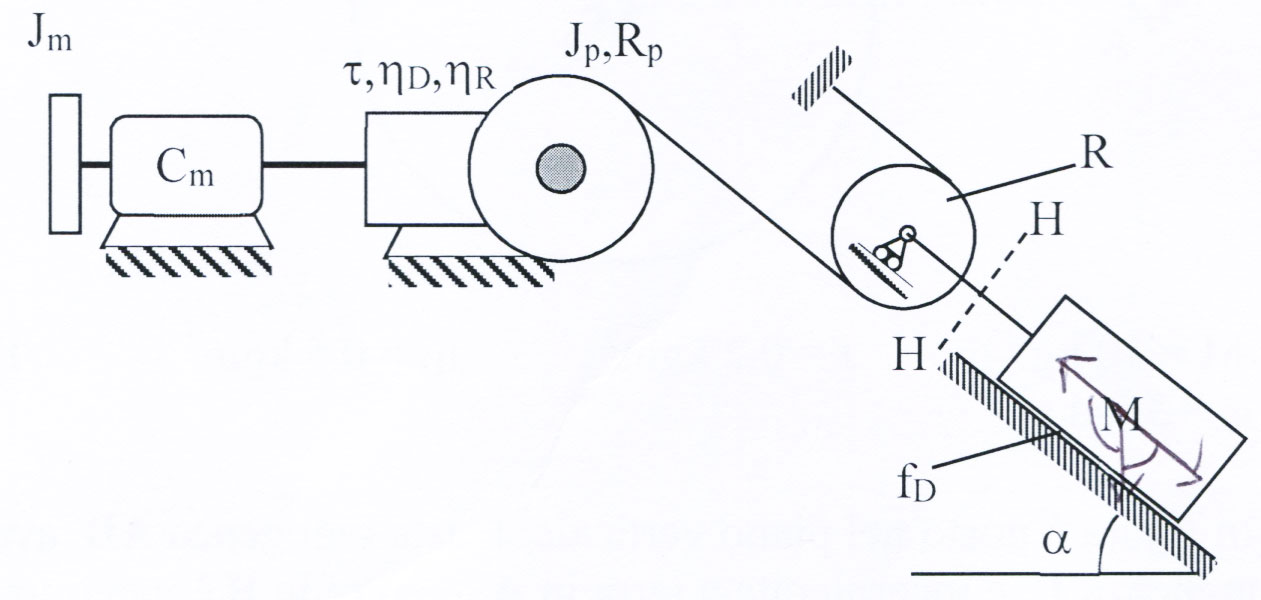
\includegraphics[width=0.75\textwidth]{2017-1109-3.jpg}
\end{figure}

\[
	M = 200\,Kg\\
	J_m = 0.04\,kgm^2\\
	J_p = 3\,kgm^2\\
	R_p = 0.25\,m\\
	R = 0.2\,m\\
\]
\[
	\tau = \dfrac{1}{25}\\
	\mu_D = 0.9\\
	\mu_R = 0.8\\
	f_D = 0.2\\
	\alpha = 30\deg
\]

L'impianto di sollevamento in figura è posto nel piano verticale ed è azionato attraverso un gruppo motore-riduttore di caratteristiche note: rapporto di riduzione $\tau$ e rendimento $\mu_D$ (per condizione di moto diretto) e $\mu_R$ (per condizioni di moto retrogrado).
All'albero di uscita della trasmissione è collegata la puleggia di raggio $R_p$ e momento di inerzia $J_p$ su cui si avvolge la fune inestensibile.
All'astra estremità, la fune si avvolge su un disco di raggio $R$ (di massa e momento di inerzia trascurabili), il cui centro è vincolato  a muoversi in direzione parallela al piano inclinato in figura, ed è infine vincolata a terra.
Al centro del disco è collegata attraverso una seconda fune una massa $M$ che si muove lungo il piano inclinato, con un coefficiente di attrito radente $f_D$.

Si chiede di calcolare:

\begin{enumerate}
\item L'accelerazione con la massa $M$ in salita, assegnata la coppia motrice erogata dal motore, pari a $C_m = 20\,Nm$.
\item La coppia motrice a regime, con la massa $M$ in salita.
\item Il tiro della fune nella sezione H-H nelle condizioni del punto 1.
\end{enumerate}

\clearpage

\subsection{Soluzione terzo esercizio (non verificata)}

\subsubsection{Primo punto}
\paragraph{Legami cinematici}
Per prima cosa identifico i legami cinematici che legano accelerazione e velocità della massa $M$ a velocità ed accelerazione angolari del motore.
\\
\\
La massa M è connessa al centro del disco di raggio $R$, e quest'ultimo individua il proprio CIR nel punto di tangenza con la corda inestensibile, che si muove alla velocità con cui la puleggia ruota.

\[
	v_p = \tau \omega_m R_p
\]

\[
	v_m = v_D = \dfrac{\tau \omega_m R_p}{2}
\]

È possibile fare un discorso analogo per le accelerazioni:

\[
	a_p = \tau \dot{\omega_m} R_p
\]

\[
	a_m = a_D = \dfrac{\tau \dot{\omega_m} R_p}{2}
\]

\paragraph{Potenza motrice}
\[
	W_m = C_m\omega_m
\]

\paragraph{Energia cinetica}

\begin{align*}
	E_c &= \dfrac{1}{2}Mv_m^2 + \dfrac{1}{2}J_m\omega_m^2 + \dfrac{1}{2}J_p(\omega_m \tau)^2\\
	      &= \dfrac{1}{2}M(\dfrac{\tau \omega_m R_p}{2})^2 + \dfrac{1}{2}J_m\omega_m^2 + \dfrac{1}{2}J_p(\omega_m \tau)^2\\
	      &= \omega_m^2(\dfrac{1}{2}M(\dfrac{\tau  R_p}{2})^2 + \dfrac{1}{2}J_m + \dfrac{1}{2}J_p(\tau)^2)\\
	      &= \dfrac{1}{2}\omega_m^2(M(\dfrac{\tau  R_p}{2})^2 + J_m + J_p(\tau)^2)\\
	      &= \dfrac{1}{2}\omega_m^2(\tau^2(\dfrac{1}{4}M R_p^2 + J_p) +  J_m)\\
\end{align*}

Derivo l'espressione così ottenuta ed ottengo:

\[
\dfrac{dE_c}{dt} =  \omega_m\dot{\omega}_m(\tau^2(\dfrac{1}{4}M R_p^2 + J_p) +  J_m)
\]

\paragraph{Tipo di moto}

\begin{align*}
	W_m - \dfrac{dE_{c_m}}{dt} &> 0\\
	C_m\omega_m -J_m\omega_m\dot{\omega}_m &> 0\\
	C_m -J_m\dot{\omega}_m &> 0\\
	20 -0.04\dot{\omega}_m &> 0\\
	\dot{\omega}_m &< 500\\
\end{align*}

Procedo assumendo il tipo di moto \textbf{diretto}, andando a verificare poi se esso rispetta la disequazione.

\paragraph{Potenza resistente}

\begin{align*}
	W_r &= \vec{F}_g\bullet\vec{v}_m + \vec{F}_d\bullet\vec{v}_m \\
	       &= F_gv_m\cos\left ( \dfrac{\pi}{2} + \dfrac{\pi}{6} \right ) + F_dv_m\cos\pi \\
	       &= -\dfrac{1}{2}F_gv_m - F_dv_m \\
\end{align*}

La forza d'attrito dinamico è definita come:

\[
	F_d = F_gf_s\cos\alpha = F_gf_s\cos\left ( \dfrac{\pi}{6} \right ) = \dfrac{\sqrt{3}}{2}F_gf_s
\]

\begin{align*}
	W_r &= -\dfrac{1}{2}F_gv_m(1-f_s\sqrt{3}) \\
		   &= -\dfrac{1}{2}Mgv_m(1-f_s\sqrt{3}) \\
		   &= -\dfrac{1}{2}Mg\dfrac{\omega_m \tau R_p}{2}(1-f_s\sqrt{3}) \\
		   &= -\dfrac{1}{4}Mg\omega_m \tau R_p(1-f_s\sqrt{3}) \\
\end{align*}

\paragraph{Potenza perduta} Essendo in condizioni di transitorio e ipotesi di moto diretto uso la formula seguente:
\[
	W_p =  -(1-\mu_D)(W_m - \dfrac{dE_{c_m}}{dt})
\]

\paragraph{Bilancio di potenze}

\begin{align*}
	W_m + W_r + W_p &= \dfrac{dE_c}{dt}\\
	W_m + W_r - (1-\mu_D)(W_m - \dfrac{dE_{c_m}}{dt}) &= \dfrac{dE_{c_m}}{dt} + \dfrac{dE_{c_r}}{dt}\\
	W_r + \mu_D(W_m - \dfrac{dE_{c_m}}{dt}) &= \dfrac{dE_{c_r}}{dt}\\
	W_r + \mu_DW_m &= \dfrac{dE_{c_r}}{dt} + \mu_D\dfrac{dE_{c_m}}{dt}\\
	\mu_DC_m\omega_m -\dfrac{1}{4}Mg\omega_m \tau R_p(1-f_s\sqrt{3}) &=  \omega_m\dot{\omega}_m(\tau^2(\dfrac{1}{4}M R_p^2 + J_p) +  \mu_DJ_m)\\
\end{align*}

\[
\dot{\omega}_m = \dfrac{\mu_DC_m -\dfrac{1}{4}Mg\tau R_p(1-f_s\sqrt{3})}{\tau^2(\dfrac{1}{4}M R_p^2 + J_p) +  \mu_DJ_m)} = 323\,rad/s^2
\]

\[
	a = \dfrac{\tau R_p \dot{\omega}_m}{2} = 1.615\,m/s^2
\]

\paragraph{Verifico ipotesi di moto diretto}

\[
	\dot{\omega}_m = 323 < 500
\]

L'ipotesi è valida.

\subsubsection{Secondo punto}
Essendo in condizioni di regime, non è più necessario considerare la variazione di energia cinetica. Il segno del coefficiente della potenza resistente, essendo in salita, è strettamente negativo, per cui il moto si mantiene diretto.

\[
	W_m + W_r + W_p = 0
\]

\[
	W_m + W_r - (1-\mu_D)W_m = 0
\]

\[
	W_r + \mu_DW_m = 0
\]

\[
	\mu_DC_m\omega_m = \dfrac{1}{4}Mg\omega_m \tau R_p(1-f_s\sqrt{3})
\]

\[
	\mu_DC_m = \dfrac{1}{4}Mg \tau R_p(1-f_s\sqrt{3})
\]

\[
	C_m = \dfrac{Mg \tau R_p(1-f_s\sqrt{3})}{4\mu_D} = 3.56\,Nm
\]

\subsubsection{Terzo punto}
Procedo con il bilancio di forze.

\begin{center}
\framebox[4in]{
\begin{minipage}[t]{3.5in}
{\Large{\danger}} \textbf{N.B.}
La forza di inerzia $Ma$ ha un verso \textbf{opposto} all'accelerazione.
\end{minipage}}
\end{center}

\[
	-Ma = F_g\sin\left ( \dfrac{\pi}{3} \right ) + \dfrac{\sqrt{3}}{2}F_gf_s - F_t
\]

\[
	-Ma = \dfrac{\sqrt{3}}{2}F_g + \dfrac{\sqrt{3}}{2}F_gf_s - F_t
\]

\[
	F_t = M(\dfrac{\sqrt{3}}{2}g(1+f_s) + a) =2361\,N
\]

\end{document}